\documentclass{article}

% {{{ Packages
        \usepackage[margin=1in]{geometry}                           % Margins
          \linespread{1.2}                                          % Increases line spacing
        \usepackage{graphicx}                                       % Image Support
          \graphicspath{ {./images/} }                              % Path to image directory
        \usepackage{color}                                          % Colors for stuff
        \usepackage{soul}                                           % Provides Highlight feature
        \usepackage{fancyhdr}                                       % Fancy Header and footer
        \usepackage{amsmath}                                        % Math support
        \usepackage{amssymb}                                        % Extended symbols for math
        \usepackage{etoolbox}                                       % IDK what it does. I just coppied it from stackexchage
          \AtBeginEnvironment{align}{\setcounter{equation}{0}}      % resets align counter for each instance
        \usepackage{listings}                                       % Code-snippet support
          % \definecolor{dkgreen}{rgb}{0,0.6,0}                     % lst-configs
          % \definecolor{gray}{rgb}{0.5,0.5,0.5}
          % \definecolor{mauve}{rgb}{0.58,0,0.82}

          % \lstset{                                                % lst-format-config
          %   frame=tb,
          %   language=Java,
          %   aboveskip=3mm,
          %   belowskip=3mm,
          %   showstringspaces=false,
          %   columns=flexible,
          %   basicstyle={\small\ttfamily},
          %   numbers=none,
          %   numberstyle=\tiny\color{gray},
          %   keywordstyle=\color{blue},
          %   commentstyle=\color{dkgreen},
          %   stringstyle=\color{mauve},
          %   breaklines=true,
          %   breakatwhitespace=true,
          %   tabsize=3
          % }
        \usepackage{caption}                                      % Caption support
        \usepackage[utf8]{inputenc}                               % utf encoding
        \usepackage{hyperref}
          \hypersetup{pdfnewwindow=true, colorlinks=false}
% }}}

% {{{ Footer section
        % Creates footer
        \pagestyle{fancy}%
        \fancyhf{}%
        \lfoot{Swapnil}%
        \cfoot{iamb4uc.xyz}%
        \rfoot{Page \thepage}%
        \renewcommand{\headrulewidth}{0pt}% Line at the head invisible
        \renewcommand{\footrulewidth}{0.9pt}% Line at the footer visible
% }}}

% {{{ Title
        \title{\Huge{\texttt{Numerical and Statistical Method}}}
        \author{\huge{by \emph{Swapnil}}\\ \\ \Large{written in {\LaTeX}}}
        \date{\today}
% }}}

\begin{document}
%{{{ Title page
      \maketitle
      \thispagestyle{empty}
      % \newpage
% }}}

%{{{ ToC
      \setcounter{tocdepth}{3}
      \tableofcontents
      \newpage
% }}}



%%%%%%%%%%%%%%%%%%%%%%%%%%%%%%%%%%%%%%%%%%%%%%%%%%%%%%%%%%%%%%%%%%%%%%%%%%%%%%%%%%%%%%%%%%%
%%%%%%%%%%%%%%%%%%%%%%%%%%%%%%%%%%%%%% Document Body %%%%%%%%%%%%%%%%%%%%%%%%%%%%%%%%%%%%%%
%%%%%%%%%%%%%%%%%%%%%%%%%%%%%%%%%%%%%%%%%%%%%%%%%%%%%%%%%%%%%%%%%%%%%%%%%%%%%%%%%%%%%%%%%%%
      % {{{
            \section*{Formula}
            {\parindent0pt

            \subsection*{$1^{st}$ order}
              $\Delta f(x)=f(x+h)-f(x)$
            
            \subsection*{$2^{nd}$ order}
              $\Delta^2 f(x)=f(x+2h)-2f(x+h)+f(x)$
            
            \subsection*{$3^{rd}$ order}
              $\Delta^3 f(x)=f(x+3h)-3f(x+2h)+2f(x+h)-f(x)$
            
            \subsection*{Newton's Forward Interpolation Formula}
              \begin{align*}
                f(x)=f(x_0)+U\Delta f(x_0) &+ \frac{U(U-1)}{2!}\Delta^2f(x_0)+\frac{U(U-1)(U-2)}{3!}\Delta^3f(x_0)\\
                                           &+ \dots+\frac{U(U-1)(U-2)\dots\{U-(n-1)\}}{n!}\Delta^nf(x_0)\\
              \end{align*}
              where $U=(\frac{x-x_0}{h})$
            
            \subsection*{Newton's backward interpolation formula}
              \begin{align*}
                f(x)=f(x_n)+U\nabla f(x_n-1) &+ \frac{U(U+1)}{2!}\nabla^2f(x_n-2)+\frac{U(U+1)(U+2)}{3!}\nabla^3f(x_n-3)\\
                                             &+ \dots+\frac{U(U+1)\dots\{U+(n-1)\}}{n!}\nabla^nf(x_0)
              \end{align*}
              where, $U=\frac{(x-x_n)}{h}$


            \subsection*{Lagrange's interpolation formula}
              \begin{align*}
                f(x)&=\frac{(x-x_1)(x-x_2)\dots(x-x_n)}{(x_0-x_1)(x_0-x_2)\dots(x_0-x_n)}f(x_0)+\frac{(x-x_0)(x-x_2)\dots(x-x_n)}{(x_1-x_0)(x_1-x_2)\dots(x_1-x_n)}f(x_1)\\
                &+ \dots +\frac{(x-x_1)(x-x_2)\dots(x-x_{n-1})}{(x_n-x_0)(x_n-x_1)\dots(x_n-x_{n-1})}f(x_n)
              \end{align*}
            
            % \subsection*{General quadrature formula}
            %   \begin{align*}
            %     I &=\int_{a=x_0}^{b=x_0+nh}f(x)dx\\
            %       &= h[ny_0+\frac{n^2}{2}\Delta y_0+(\frac{n^3}{3}-\frac{n^2}{2})\frac{\Delta^2y_0}{2!}+(\frac{n^4}{4}-n^3-n^2)\frac{\Delta^3y_0}{3!}\\
            %       &+ \dots+upto\ (n+1)\ terms]
            %   \end{align*}
            
            \subsection*{Trapezoidal Rule}
              \begin{align*}
                \int_{x_0}^{x_0+nh}f(x)dx = h[(\frac{y_0+y_n}{2})+(y_1+y_2+y_3+\dots+y_{n-1})]
              \end{align*}

            \subsection*{Simpsons $\frac{1}{3}^{rd}$ Rule}
              \begin{align*}
                \int_{x_0}^{x_0+nh}f(x)dx &= \frac{h}{3}(y_0+y_n)+4(y_1+y_3+\dots+y_{n-1})+2(y_2+y_4+\dots+y_{n-2})
              \end{align*}
            
            \subsection*{Simpsons $\frac{3}{8}^{th}$ Rule}
              \begin{align*}
                \int_{x_0}^{x_0+nh}f(x)dx=\frac{3h}{8}[(y_0+y_n) &+ 3(y_1+y_2+y_4+y_5+\dots+y_{n-1})\\
                                                                 &+ 2(y_3+y_6+\dots+y_{n-3})]
              \end{align*}
            
            }
            
            \newpage

            \section{Calculas of finite difference}
              The calculas of finite difference deals with the changes in the values of the 
              dependent variable due to the changes in the independent variable.
              
              Let, `$y$' be a function of `x' represented by $y=f(x)$. Let, $a,a+h,a+2h,
              \dots,(a+nh)$ be the $(n+1)$ equidistant values of x and 
              $f(a),f(a+h),f(a+2h),\dots,f(a+nh)$ be the corresponding values of $f(x)$.
              
              The values of $x$ are called arguments and the values of $f(x)$ are called 
              entries.
              
              Again,

              \begin{align*}
                (a+h)-a&=(a+2h)-(a+h)=(a+3h)-(a+2h)=\dots\\
                &=(a+nh)-\{a+(n-1)h\}\\
                &=h
              \end{align*}

              where, `h' is called the interval of differences.

              \begin{enumerate}
                \item Difference of first order($\Delta$)
                  
                  \begin{equation*}
                    \Delta f(x)=f(x+h)-f(x)
                  \end{equation*}
                
                \item Difference of second order($\Delta^2$)
              
                  \begin{align*}
                    \Delta^2 f(x)&=\Delta \{\Delta f(x)\}\\
                    &=\Delta \{f(x+h)-f(x)\}\\
                    &=\Delta f(x+h)-\Delta f(x)\\
                    &=f(x+2h)-f(x+h)-\{f(x+h)-f(x)\}\\
                    \Delta^2f(x)&=f(x+2h)-2f(x+h)+f(x)\\
                  \end{align*}
              
                \item Difference of second order($\Delta^3$)
              
                  \begin{align*}
                    \Delta^3 f(x)&=\Delta \{\Delta^2 f(x)\}\\
                    &=\Delta \{f(x+2h)-2f(x+h)+f(x)\}\\
                    &=f(x+3h)-f(x+2h)-2f(x+2h)+2f(x+h)+f(x+h)-f(x)\\
                    &=f(x+3h)-3f(x+2h)+2f(x+h)-f(x)
                  \end{align*}
              
              \end{enumerate}
            
            
            \section{Difference Table}
              When we arrange the difference of various orders of a function systematically 
              along with arguments and entries in a table, then its is known as diffrence table.
              
              Let, $x_0,x_1,x_2,x_3$ are 4 equidistant values of x such that $x_1-x_0,x_2-x_1,x_3-x_2=h$
              and $f(x_0),f(x_1),f(x_2),f(x_3)$ are the corresponding values of $f(x)$,
              then the difference table is
              
              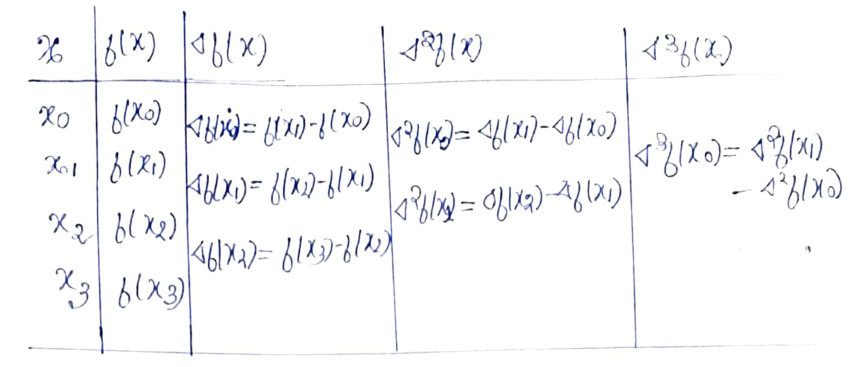
\includegraphics[scale=0.65]{difference table}
            
            
            \section{Interpolation}
              Interpolation is a technique of estimating the approximates of the value 
              of the depending variable corresponding to a value of the independent variable, 
              between its two extreme values, on the basis of the given independent and 
              dependent variables values.
            
            \section{Assumption of interpolation}
              The application of principal of interpolation is subject to the following assumption.
              \begin{itemize}
                \item There is no sudden jumps in figures from one period to another period.
                  
                \item The rate of change of figure is uniform, over-time.
              
              \end{itemize}
            \section{Different Interpolation formulae}
              \subsection{Newton's forward interpolation formula}
                It is used to estimate the value of the dependent variable corresponding to 
                a given value of the independent variable, if:

                \begin{enumerate}
                  \item The independent variable $x$, increases by equal intervals.
                  \item The value of $x$, correponing which the value of $y$ us to be interpolated in the first hub of the series.  
                \end{enumerate}

                The formula is 

                \begin{align*}
                  f(x)=f(x_0)+U\Delta f(x_0)&+\frac{U(U-1)}{2!}\Delta^2f(x_0)+\frac{U(U-1)(U-2)}{3!}\Delta^3f(x_0)\\
                  &+\dots+\frac{U(U-1)(U-2)\dots\{U-(n-1)\}}{n!}\Delta^nf(x_0)\\
                \end{align*}

                where $U=(\frac{x-x_0}{h})$ and h is the interval of differencing.
                
                % \subsubsection{Derivation}{{{
                % Let, $y=f(x)$, be a function,
                
                % Here, the argument's $x_0,x_1,\dots.x_n$ are equidistant. $x_1-x_0=x_2-x_1=\dots=x_n-x_{n-1}=h$
                
                % Let us take a polynomial of $n^{th}$ degree as our interpolation formula.
                
                % Let 
                % \begin{equation}\label{dv1}
                %   f(x)=a_0+a_1(x-x_0)+a_2(x-x_0)(x-x_1)+\dots+a_3(x-x_0)(x-x_1)\dots(x-x_{n-1})
                % \end{equation}
                % where $a_0,a_1,\dots,a_n$ are the constants to be determined.
                
                % Now, putting $x=x_0$ in equation number (\ref{dv1}) 
                % \begin{align*}
                %   f(x_0)&=a_0
                % \end{align*}
                % Again, putting $x=x_1$ in equation (\ref{dv1})
                % \begin{align*}
                %   f(x_1)&=a_0+a_1(x_1-x_0)\\
                %   \Rightarrow f(x_1)&=f(x_0)+a_1*h\\
                %   \Rightarrow a_1 &=\frac{f(x_1)-f(x_0)}{h}\\
                %   &=\frac{\Delta f(x_0)}{h}
                % \end{align*}
                
                % Again, putting $x=x_2$ in equation (\ref{dv1})
                % \begin{align*}
                %               f(x_2)  &= a_0+a_1(x_2-x_0)+a_2(x_2-x_0)(x_2-x_1)\\
                %   \Rightarrow f(x_2)  &= f(x_0)+\frac{\Delta f(x_0)}{h}(x_2-x_1+x_1-x_0)\\ &+ a_2(x_2-x_1+x_1-x_0)(x_2-x_1)\\
                %   \Rightarrow f(x_2)  &= f(x_0)+\frac{\Delta f(x_0)}{h}*2h+a_2*2h*h\\
                %   \Rightarrow f(x_2)  &= f(x_0)+2\Delta f(x_0)+2h^2a_2\\
                %   \Rightarrow a_2     &= \frac{f(x_2)-2\Delta f(x_0)-f(x_0)}{2h^2}\\
                %   \Rightarrow a_2     &= \frac{f(x_2)-2f(x_1)+2f(x_0)-f(x_0)}{2h^2}\\
                %                       &= \frac{f(x_2)-2f(x_1)+f(x_0)}{2!h^2}\\
                %                       &= \frac{\Delta^2 f(x_0)}{2!h^2}
                % \end{align*}
                
                % Again, putting $x=x_3$ is equation (\ref{dv1})
                % \begin{equation*}
                %   a_3=\frac{\Delta^3f(x_0)}{3!h^3}\\
                % \end{equation*}
                
                % ....................
                
                % ....................................
                
                
                % Similarly, putting $x=x_n$ in equation (\ref{dv1})
                % \begin{equation*}
                %   a_n=\frac{\Delta^nf(x_0)}{n!h^n}
                % \end{equation*}
                
                % Now putting the value of $a_0,a_1,a_2,a_3,\dots,a_n$ in equation (\ref{dv1}), we get,
                % \begin{equation*}\label{dv2}
                %   f(x)=f(x_0)+\frac{\Delta f(x_0)}{h}(x-x_0)+\frac{\Delta^2f(x_0)}{2!h^2}(x-x_0)(x-x_1)
                % \end{equation*}
                % \begin{equation*}\label{dv2}
                %       +\frac{\Delta^3f(x_0)}{3!h^3}(x-x_0)(x-x_1)(x-x_2)
                % \end{equation*}
                % \begin{equation}\label{dv2}
                %       +\dots+\frac{\Delta^nf(x_0)}{n!h^n}(x-x_0)(x-x_1)\dots(x-x_{n-1})
                % \end{equation}
                
                % Let us put $U=\frac{x-x_0}{h}$ in equation (\ref{dv2})
                % \begin{align*}
                %   f(x)&=f(x_0)+U\Delta f(x_0)+\frac{U(U-1)}{2!}\Delta^2f(x_0)+\frac{U(U-1)(U-2)}{3!}\Delta^3f(x_0)\\
                %   &+\dots+\frac{U(U-1)\dots\{U-(n-1)\}}{n!}\Delta^nf(x_0)
                % \end{align*}}}}
              
              \subsection{Newton's backward interpolation formula}
                Let, $f(x)$ be a polynomial  of degree $n$ and $n+1$ equidistant values of $x$ along then
                corresponding values of $f(x)$. The Newton's backward interpolation formula is

                \begin{align*}
                  f(x) &= f(x_n)+U\nabla f(x_n-1)+\frac{U(U+1)}{2!}\nabla^2f(x_n-2)+\frac{U(U+1)(U+2)}{3!}\nabla^3f(x_n-3)\\
                       &+\dots+\frac{U(U+1)\dots\{U+(n-1)\}}{n!}\nabla^nf(x_0)
                \end{align*}
              
                where, $U=\frac{(x-x_n)}{h}$, where h is the interval of differences.
                
                The Newton's backward interpolation formula is used to estimate values of the dependent 
                variable corresponding to a given value of the independent variable.

                \begin{enumerate}
                  \item The independent variable $x$ increases by equal intervals.
                  \item The value of $x$ corresponding to each value of $y$ is to be interpolated in 
                    the $2^{nd}$ half of the series.
                \end{enumerate}
              
              \subsection{Lagrenge's interpolation formula}
              Let, $f(x_0),f(x_1),\dots,f(x_n)$ be the entries corresponding to the argument 
              $x_0,x_1,\dots,x_n$ which are not necessarily in equal intervals. The interpolation 
              formula given by Lagrenge to estimate the value of $y$ corresponding to a value of $x$ 
              between any two consecutive values of the given values is

              \begin{align*}
                f(x)&=\frac{(x-x_1)(x-x_2)\dots(x-x_n)}{(x_0-x_1)(x_0-x_2)\dots(x_0-x_n)}f(x_0)+\frac{(x-x_0)(x-x_2)\dots(x-x_n)}{(x_1-x_0)(x_1-x_2)\dots(x_1-x_n)}f(x_1)\\
                &+ \dots +\frac{(x-x_1)(x-x_2)\dots(x-x_{n-1})}{(x_n-x_0)(x_n-x_1)\dots(x_n-x_{n-1})}f(x_n)
              \end{align*}

              Lagrange's Interpolation formula is usually and when the values of the independent
              variable $x$ are not equidistant. To apply Lagrange's formula the value of $x$ 
              corresponding to which the value of $y$ is to be interpolated may be anywhere in 
              between the first and last terms.
              
              To apply Lagrange's formula, constuction of difference table is not needed.
            
            \section{Numerical Integration}
              Numerical Integration is the process of finding or evaluating definate integral is 
              
              $I=\int_{a}^{b}f(x)dx$ from a set of numerical value of the integrant $f(x)$. 
              If it is applied to the integration of a function of a single variable then the 
              process is known as quadrature. The problem of numerical integration is solved by 
              first approximating the integrant by a polynomial with the help of an interpolation 
              formula and then integrating this expression between the desired limits.
              
              \begin{align*}
                \int xdx&=\frac{x^2}{2}\\
                \int x^ndx&=\frac{x^{n+1}}{n+1}
              \end{align*}
            
            % \subsection{General quadrature formula}{{{
            % Let $y=f(x)$ be the given integrant and the corresponding integral is 
            % \begin{equation*}
            %   I=\int_{a=x_0}^{b=x_0+nh}f(x)dx
            % \end{equation*}
            % Let us suppose that we are given a set of numerical values of the integrant corresponding to some equidistant values of $x$.
            
            % Let us divide the range $(a,b)$ in $n$ equal parts, each of which with is $nh$ i.e. $b-a=nh$.
            
            % \noindent Say $a=x_0, a+h=x_0+h,\dots a+nh=x_0+nh$
            
            % Let us take the Newton's Forward Interpolation Formula as an approximating of $f(x)$.
            
            % \begin{align*}
            %   \because I=\int_{a=x_0}^{b=x_0+nh}f(x)dx\\
            % \end{align*}
            
            % \begin{align*}
            %   =\int_{x_0}^{x_0+nh}f(x_0)+U\Delta f(x_0) &+ \frac{U(U-1\Delta^2f(x_0))}{2!}+\frac{U(U-1)(U-2)}{3!}\Delta^3f(x)\\
            %                                               &\dots\frac{U(U-1)(U-2)\dots\{U-(n-1)\}}{n!}\Delta^nf(x_0)
            % \end{align*}
            
            % \begin{align*}
            %   =\int_{x_0}^{x_0+nh}y_0+\Delta y_0+\frac{U(U-1)}{2!}\Delta^2y_0 &+ \frac{U(U-1)(U-2)}{3!}\Delta^3y_0\\
            %                                                                   &+ \dots+\frac{U(U-1)\dots\{U-(n-1)\}}{n!}\Delta^ny_0\}dx
            % \end{align*}
            % where,
            % \begin{align*}
            %               U &= \frac{x-x_0}{h}\\
            %   \Rightarrow x &= x_0+hu\\
            %   \Rightarrow \frac{dx}{du} &= 0+h\frac{d(u)}{du}=h\\
            %   \Rightarrow dx &= hdu
            % \end{align*}
            % when, $x=x_0$, $U=\frac{x_0-x_0}{h}=0$
            
            % \noindent where, $x=(x_0+nh)$, $U=\frac{x_0+nh-x_0}{h}=\frac{nh}{h}=n$
            
            % \begin{align*}
            %   I &= \int_{0}^{n}\{y_0+U\Delta y_0+\frac{U^2-U}{2!}\Delta^2y_0+\frac{U^3-3U^2+2U}{3!}\Delta^3y_0\\
            %     &+ \dots +\ upto\ (n+1)\ terms\} hdu\\
            %     \ \\
            %     &= h[y_0U+\Delta y_0\frac{U^2}{2}+\frac{\Delta^2y_0}{2!}(\frac{U^3}{3}-\frac{U^2}{2})+\frac{\Delta^3y_0}{3!}(\frac{U^4}{4}-\frac{U^3}{3}+\frac{U^2}{2})\\
            %     &+ \dots+upto\ (n+1)\ terms]_{0}^{n}\\
            %     \ \\
            %     &= h[ny_0+\frac{n^2}{2}\Delta y_0+(\frac{n^3}{3}-\frac{n^2}{2})\frac{\Delta^2y_0}{2!}+(\frac{n^4}{4}-n^3-n^2)\frac{\Delta^3y_0}{3!}\\
            %     &+ \dots+upto\ (n+1)\ terms]
            % \end{align*}
            
            % This is called the general quadrature formula.}}}
            
            \subsection{Trapezoidal Rule}
              The general quadrature formula is

              \begin{align*}
                I &=\int_{a=x_0}^{b=x_0+nh}f(x)dx\\
                  &= h[ny_0+\frac{n^2}{2}\Delta y_0+(\frac{n^3}{3}-\frac{n^2}{2})\frac{\Delta^2y_0}{2!}+(\frac{n^4}{4}-n^3+n^2)\frac{\Delta^3y_0}{3!}
              \end{align*}

              \begin{align}\label{dv3}
                  &+ \dots+upto\ (n+1)\ terms]
              \end{align}
              
              Putting $n=1$ in equation number \ref{dv3}, and neglecting all the differece 
              higher than 1, we get:
              
              \begin{align*}
                I_1 &= \int_{x_0}^{x_0+h}f(x)dx\\
                    &= h[y_0+\frac{1}{2}\Delta y_0]\\
                    &= h[y_0+\frac{1}{2}(y_1-y_0)]\\
                    &= h[\frac{2y_0+y_1-y_0}{2}]\\
                    &= h[\frac{y_0+y_1}{2}]
              \end{align*}
              
              Similarly,
              
              \begin{align*}
                I_2 &= \int_{x_0+h}^{x_0+2h}f(x)dx = h[\frac{y_1+y_2}{2}]
              \end{align*}
              
              \begin{align*}
                I_3 &= \int_{x_0+2h}^{x_0+3h}f(x)dx = h[\frac{y_2+y_3}{2}]
              \end{align*}
              \dots 
              
              \dots 
              \begin{align*}
                I_n &= \int_{x_0+(n-1)h}^{x_0+nh}f(x)dx = h[\frac{y_{(n-1)}+y_n}{2}]
              \end{align*}
              
              Adding these n integrals we get
              \begin{align*}
                \int_{x_0}^{x_0+nh}f(x)dx &= h[(\frac{y_0-y_1}{2})+(\frac{y_1-y_2}{2})+\dots+(\frac{y_{(n-1)}+y_n}{2})]\\
                                          &= h[(\frac{y_0+y_n}{2})+(y_1+y_2+y_3+\dots+y_{n-1})]
              \end{align*}
              
              This is called the Trapezoidal Rule.
              
              \pagebreak
              \textbf{Condition for validity of trapezoidal rule}
              \begin{enumerate}
                \item $f(x)$ should be a polynomial of degree of 1, i.e. a 
                  straight line of the form $f(x)=a+bx$
                \item The value of $x$ should be equidistant
                \item The number of divisions of the integral $(x_0,x_0+nh)$ 
                  should be multiple of 1, like 3, 5, 7, etc.
              \end{enumerate}
            
            \subsection{Simpson's $\frac{1}{3}^{rd}$ rule}
              The general quadrature formula is 

              \begin{align*}
                I &=\int_{a=x_0}^{b=x_0+nh}f(x)dx\\
                  &= h[ny_0+\frac{n^2}{2}\Delta y_0+(\frac{n^3}{3}-\frac{n^2}{2})\frac{\Delta^2y_0}{2!}+(\frac{n^4}{4}-n^3+n^2)\frac{\Delta^3y_0}{3!}\\
                  &+ \dots+upto\ (n+1)\ terms]
              \end{align*}

              Putting $n=2$ and neglecting all the differences higher then second order.

              \begin{align*}
                I_1=\int_{a=x_0}^{b=x_0+2h}f(x)dx &= h[2y_0+2\Delta y_0+(\frac{8}{3}-2)\frac{\Delta^2y_0}{2!}]\\
                                                  &= h[2y_0+2(y_1-y_0)+(\frac{8}{3}-2)\frac{y_2-2y_1+y_0}{2}]\\
                                                  &= h[2y_0+2y_1-2y_0+\frac{2}{3}*\frac{y_2-2y_1+y_0}{2}]\\
                                                  &= h[2y_1+\frac{y_2-2y_1+y_0}{3}]\\
                                                  &= h[\frac{6y_1+y_2-2y_1+y_0}{3}]\\
                                                  &= h[\frac{y_0+4y_1+y2}{3}]\\
                                                  &= \frac{h}{3}(y_0+4y_1+y_2)
              \end{align*}
              
              Simillarly,
              
              \begin{align*}
                I_4=\int_{x_0+2h}^{x_0+4h}f(x)dx &= \frac{h}{3}(y_2+4y_3+y_4)
              \end{align*}

              And,

              \begin{align*}
                I_n=\int_{x_0+(n-2)h}^{x_0+nh}f(x)dx &= \frac{h}{3}(y_{n-2}+4y_{n-1}+y_n)
              \end{align*}
              
              On adding all these integrals, we get:
              
              \begin{align*}
                \int_{x_0}^{x_0+nh}f(x)dx &= \frac{h}{3}(y_0+y_n)+4(y_1+y_3+\dots+y_{n-1})+2(y_2+y_4+\dots+y_{n-2})
              \end{align*}

              This formula is known as Simpson's $\frac{1}{3}^{rd}$ formula.
              
              \textbf{Condition for validity of Simpson's $\frac{1}{3}^{rd}$ rule.}

              \begin{enumerate}
                \item $f(x)$ should be a polynomial of degree 2 of the form $f(x)=a+bx+cx^2$
                \item The values of x should be equidistant
                \item The number of division of the interval $(x_0,x_0+nh)$ should be multiple of 2 like 2, 4, 6, 8, 10, etc.
              \end{enumerate}
            
            \subsection{Simpson's $\frac{3}{8}^{th}$ rule}
              The general quadrature formula is 

              \begin{align*}
                I &=\int_{a=x_0}^{b=x_0+nh}f(x)dx\\
                  &= h[ny_0+\frac{n^2}{2}\Delta y_0+(\frac{n^3}{3}-\frac{n^2}{2})\frac{\Delta^2y_0}{2!}+(\frac{n^4}{4}-n^3+n^2)\frac{\Delta^3y_0}{3!}\\
                  &+ \dots+upto\ (n+1)\ terms]
              \end{align*}

              Putting $n=3$ and neglicting all the difference higher than $3^{rd}$ order.

              \begin{align*}
                I_1=\int_{x_0}^{x_0+3h}f(x)dx &= h[3y_0+\frac{3}{2}\Delta y_0+(\frac{27}{3}-\frac{9}{2})\frac{\Delta^2y_0}{2!}+(\frac{81}{4}-27+9)\frac{\Delta^3y_0}{3!}]\\
                                        &= h[3y_0+\frac{3}{2}(y_1-y_0)+(9-\frac{9}{2})(\frac{y_2-2y_1+y_0}{2})+(\frac{81}{4}-27+9)\\
                                        &  (\frac{y_3-3y_2+3y_1-y_0}{6})]\\
                                        \ \\ 
                                        &= h[3y_0+\frac{9}{2}(y_1-y_0)+\frac{9}{3}(\frac{y_2-2y_1+y_0}{2})+\frac{3}{8}(y_3-3_2+3y_1-y_0)]\\
                                        &= \frac{3h}{8}[8y_0+12(y_1-y_0)+6(y_2-2y_1+y_0)+(y_3-3y_2+3y_1-y_0)]\\
                                        &= \frac{3h}{8}[y_0+3y_1+3y_2+y_3]\\
              \end{align*}
              
              Similarly,
              
              \begin{align*}
                \int_{x_0+3h}^{x_0+6h}f(x)dx &= \frac{3h}{8}[y_3+3y_4+3y_5+y_6]\\
              \end{align*}
              \dots
              
              \dots
              \begin{align*}
                \int_{x_0+(n-3)h}^{x_0+nh}f(x)dx &= \frac{3h}{8}[y_{n-3}+3y_{n-2}+3y_{n-1}+y_n]\\
              \end{align*}
              
              Adding all the integrals,
              
              \begin{align*}
                \int_{x_0}^{x_0+nh}f(x)dx=\frac{3h}{8}[(y_0+y_n) &+ 3(y_1+y_2+y_4+y_5+\dots+y_{n-1})\\
                                                                 &+ 2(y_3+y_6+\dots+y_{n-3})]
              \end{align*}

              This formula is known as Simpson's $\frac{3}{8}^{rd}$ formula.
              
              \textbf{Conditions for validity of Simpson's $\frac{3}{8}^{rd}$ rule.}

              \begin{enumerate}
                \item $f(x)$ should be a polynomial of degree 3 of the form 
                  $f(x)=a+6x+cx^2+dx^3$
                \item The value of $x$ should be equidistant.
                \item The number of division of the interval $(x_0,x_0+nh)$
                  should be multiple of 3 like 3, 6, 9, etc.
              \end{enumerate}

    % }}}


%%%%%%%%%%%%%%%%%%%%%%%%%%%%%%%%%%%%%%%%%%%%%%%%%%%%%%%%%%%%%%%%%%%%%%%%%%%%%%%%%%%%%%%%%%%%
\end{document}
